\subsection{Sprint 2: Twisted and peer discovery}
In the second sprint, a networking library called Twisted is integrated into tsukiji. Instead of hardcoding peers, a peer discovery mechanism is introduced. Finally, a gossip protocol replaces the broadcasting protocol.

\subsubsection{Twisted}
\label{sprint2:twisted}
The networking protocol using raw sockets of sprint 1 showed how the idea of the implementation would work in practice.
What we need now is a stable and well-tested implementation to further our project into scaling and to prepare it for the real deal.
To save us the work required to produce such code, we chose to use a library instead.

Twisted \cite{twisted} is a open source library that offers many options for networking and communication. 
Their site describes it as an event-based framework for internet applications. Using this framework, rather than our self-made code had a couple of benefits:
\begin{itemize}
\item Twisted is well-tested.
\item Twisted is event-driven.
\item Twisted has an implementation of the UDP protocol.
\item Twisted is already implemented.
\end{itemize}
The current implementation of the broadcasting protocol of sprint 1 does not contain any tests so there is no guarantee that the code is bug-free and ready to be extended.
Twisted on the other hand has numerous test cases that cover many use-cases.
Because of this, a lot of time can be saved by trusting that the imported functions of Twisted will behave as promised instead of writing tests for our own implementation.

The current implementation uses a threaded approach to handling requests.
Threads are not maintained particularly well and are an enormous strain on the processor.
Twisted gives a structure that requires a low amount of recourses when it is not handling data for sending or receiving messages with an event-driven engine.

Torrenting networks generally use the UDP transport protocol to carry their data.
The reason for this is that, compared to TCP, UDP traverses more easily over NAT and firewalls.
Keeping in line with this, it would be useful to have a similar way of handling communication in extensions of these programs.
Twisted provides options for both TCP and UDP.

All of the issues above could be made and added to the implementation made in the previous sprint.
However, this would cost a lot of time that could be spent on solving other issues.

Given these advantages, Twisted seems like a great way to improve the current networking implementation and provide reliability and scalability.

\subsubsection{Peer discovery}
\label{sprint2:peerdiscovery}
One issue of having a decentralised system is that there is no central authority that can provide information about all the users and all the data. 
Because of this, when a peer is not yet part of the network, it has no knowledge of who to contact for more information about the network and all the peers connected to it. 
This problem of peer discovery has not yet been solved in a truly decentralised way. 
The current solution is to bootstrap a user by giving them a peerlist.
This peerlist contains a number of "super peers" that should always be online.
The new peer then connects with one random super peer.
This super peer sends a list of other peers back to the new peer.
Now the new peer knows about who is in the network.
From now on, the exchanging of peer lists does not necessarily have to occur with a super peer, but can also occur with other, normal peers.
With this implementation, the system is mostly decentralised, but it still requires a number of super peers to be online to support any initial connections of new users.

\subsubsection{Gossip}
\label{sprint2:gossip}
The implementation of sprint 1 used the broadcasting protocol, where every peer is connected to every other peer.
This protocol is easy to implement but does not scale well. 
When the network grows larger, every peer has more recipients to contact and there are more peers sending messages all around.
To increase scalability, a better protocol is required.
\begin{figure}[H]
  \centering
  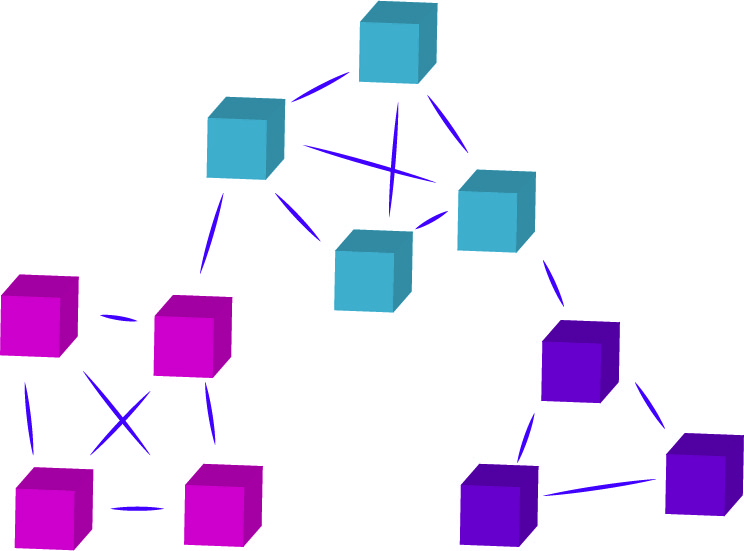
\includegraphics[width=\textwidth]{gossip}
  \caption{Gossip: The color of the cubes represent the groups of the peers and the lines represent connections between peers}
  \label{gossipfig}
\end{figure}
The peer discovery discussed in the previous section inherently creates a situation where subgroups of peers are created that know of each other.
A peer can be in multiple groups and they provide the connection between groups.
The collection of groups connected to each other is called a clique.
This property of the network is exactly what an epidemic or gossip protocol uses.
In this type of protocol, a peer relays all the messages it receives to all peers in its group, which eventually spreads through the entire clique, as shown in figure \ref{gossipfig}.
Since the peers in a group have randomly chosen who sends them their peerlist, every peer should have a slightly different group.
Even in the case that every peer only encounters users within its own subgroup, the original master-peers can still act as a bridge between the groups.

Using the gossip protocol severely reduces network traffic compared to the broadcasting protocol.
The addition of a new user now only increases the load of one group, rather than of the entire network.
With the addition of many new peers, new groups will form to cut down the overall stress.
This protocol has proven itself to be scalable \cite{voulgaris2005robust}.